Before diving into details, we demonstrate a particular application of the proposed framework. Specifically, we shall perform stochastic PTA of a dual-core platform, wherein the parameters that affect the leakage current are uncertain. The application is a part of the illustrative example in \sref{illustrative-example} and, therefore, will be described in details later on.

\begin{figure}
  \centering
  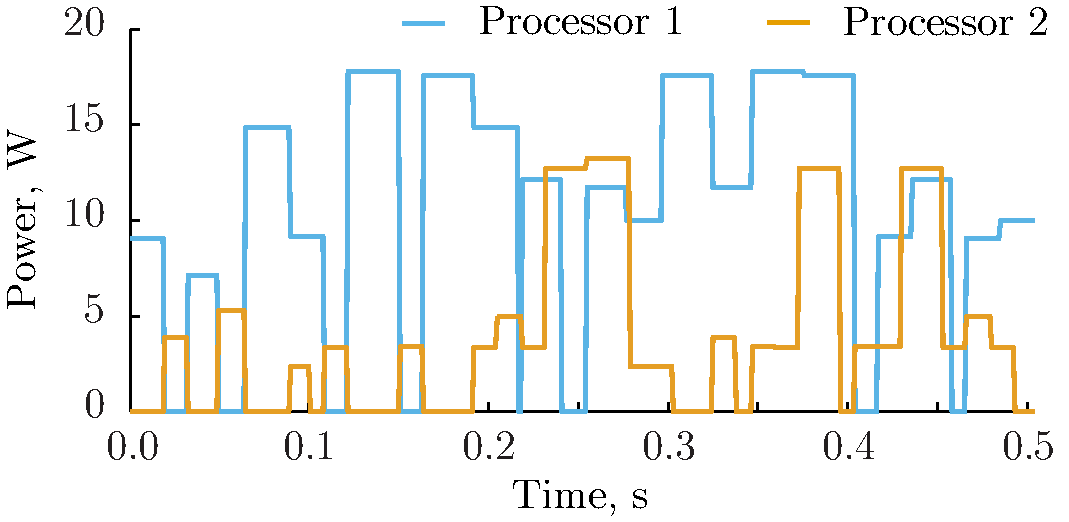
\includegraphics[width=1.00\columnwidth]{include/assets/application-power.pdf}
  \vspace{-0.5em}
  \caption{A dynamic power profile.}
  \flabel{application-power}
  \vspace{-0.5em}
\end{figure}

\begin{figure}[bl]
  \vspace{-1.0em}
  \centering
  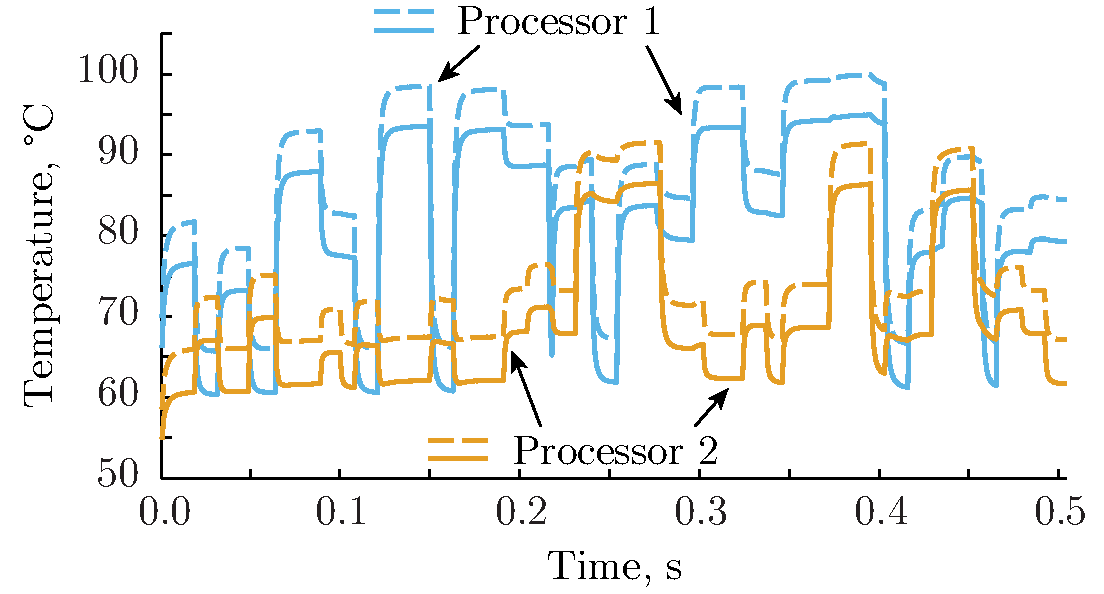
\includegraphics[width=0.90\columnwidth]{include/assets/application-temperature.pdf}
  \vspace{-0.5em}
  \caption{The expected temperature (the solid lines) and one standard deviation above it (the dashed lines).}
  \flabel{application-temperature}
\end{figure}

Without loss of generality, we address one of the most critical leakage parameters: the effective channel length \cite{chandra2010, juan2011, juan2012, srivastava2010, shen2009}. Due to process variation, the channel length is a \rv, which we denote by $\Leff(\o)$. The variations of $\Leff(\o)$ are split into global $\gLeff(\o)$ and local $\lLeff(\o)$ parts. Assume $\gLeff(\o)$ is shared among the processors whereas each processor has its own local \rv\ $\lLeff_i(\o)$. Therefore, the channel length of the $i$th processor is
\begin{equation} \elabel{leakage-partition}
  \Leff_i(\o) = \nLeff + \gLeff(\o) + \lLeff_i(\o)
\end{equation}
where $\nLeff$ is the nominal value. Consequently, the uncertain parameters $\vU(\o)$ of the problem have been identified, \ie,
\[
  \vU(\o) = \vec{\lLeff_1(\o), \; \lLeff_2(\o), \; \gLeff(\o) }.
\]
The variations of $\Leff(\o)$ can be accurately approximated by Gaussian distributions \cite{juan2011, juan2012, srivastava2010}; hence, we assume that $\vU(\o)$ is a Gaussian vector with a given covariance matrix. Since the local \rvs\ are known to have spacial correlations, the uncertain parameters $\vU(\o)$ are not independent. Therefore, at \stage{1}\ of the framework, we transform $\vU(\o)$ into a set of independent \rvs\ denoted by $\vZ(\o) = \vec{\Z_1(\o), \; \Z_2(\o)}$. Note, due to the correlations between $\lLeff_i(\o)$, we were also able to perform model order reduction to two \rvs. At \stage{2}, we decide on the power model; assume it is
\begin{align*}
  & \P_i(\t, \o) = \P_{\dyn, i}(\t) + \beta_i \: \exp \left(\vphantom{\T^2_i} \alpha_0 + \alpha_1 \: \Leff_i(\o) \right. \\
  & \qquad {} + \left. \alpha_2 \: \T_i(\t, \o) + \alpha_3 \: \Leff_i(\o) \: \T_i(\t, \o) + \alpha_4 \: \T_i(\o, \t)^2 \right),
\end{align*}
for $i = 1, 2$, which is a measurement- or simulation-based model of the corresponding electrical circuits where $\alpha_j, \beta_i$ are some fitting coefficients. Note, however, the power model is irrelevant to our framework; in \fref{algorithm}, it is denoted by a ``black-box'' function $\f$. We move on to the thermal model, \stage{3}. The thermal specification $\system$ of the system at hand is assumed to be given; in particular, the floorplan of the die and the configuration of the thermal package are known. Therefore, we construct an equivalent RC thermal circuit of the system, which is depicted in \fref{circuit} in the appendix. Hence, a mathematical model of heat transfer within the platform is acquired. We transform this model in a certain way and denote the result by $\mCF(\t)$ and $\mCS(\t)$ in \fref{algorithm}. At \stage{4}, given a nominal dynamic power profile $\profPdyn$, the independent \rvs, power model, and thermal model are fused together to produce the corresponding stochastic power $\profP{\o}$ and temperature $\profT{\o}$ profiles. The stochastic profiles are nothing more than two polynomials of $\Z_1(\o)$ and $\Z_2(\o)$ with time-dependent coefficients. For example, assuming a second-total-order PC expansion, the temperature at the $k$th moment of times is
\begin{align*}
  \vTO_k(\o) &= \pccs_{k1} + \pccs_{k2} \Z_1(\o) + \pccs_{k3} \Z_2(\o) + \pccs_{k4} \Z_1(\o) \Z_2(\o) \\
  & \qquad \qquad {} + \pccs_{k5} (\Z_1(\o)^2 - 1) + \pccs_{k6} (\Z_2(\o)^2 - 1)
\end{align*}
where $\pccs_{ki}$ are vectors with two elements corresponding to the two processors. The expansion for power has the same structure but different coefficients. Such a series might be shorter or longer depending on the accuracy requirements. As we see, our surrogate model has a negligibly small computational cost at \stage{5}: for any outcome of the uncertain parameters $\vZ(\o) \equiv \vZ$, we can plug it into the above equation and easily compute the corresponding temperature; the same applies for power. Furthermore, the expectation and variance are calculated as simple as
\[
  \oExp{\vTO_k(\o)} = \pccs_{k1} \hspace{1em} \text{and} \hspace{1em} \oVar{\vTO_k(\o)} = \sum_{i = 2}^{6} \pcn_i \: \pccs_{ki}^2
\]
where $\pcn_i$ are normalization constants, and the squaring should be understood element-wise. For instance, assume the power profile of the system is the one shown in \fref{power}. Then, after the computations at \stage{4}, we get the corresponding stochastic temperature profile and can observe its expectation and standard deviation, which are shown in \fref{temperature}. The displayed curves closely match those obtained by MC simulations with $10^4$ samples; however, our method takes less than a second, on a personal computer, while the MC-based approach takes more than a day as we shall discuss in \sref{experimental-results}.
